\documentclass[tikz,border=10pt]{standalone}
\begin{document}
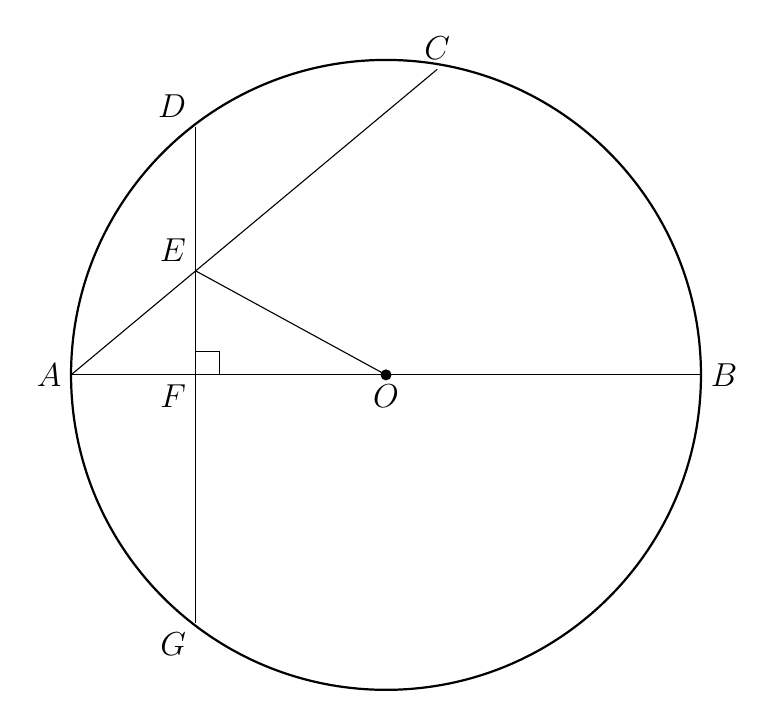
\begin{tikzpicture}[scale=1, every node/.style={font=\large}]
  % Circle
  \coordinate (O) at (0,0);
  \draw[thick] (O) circle (4);

  % Points
  \coordinate (A) at (-4,0);
  \coordinate (B) at (4,0);
  \coordinate (F) at (-2.416,0);
  \coordinate (D) at (-2.416,3.147);
  \coordinate (G) at (-2.416,-3.147);
  \coordinate (E) at (-2.416,1.32);
  \coordinate (C) at (0.65,3.88);

  % Lines
  \draw (A) -- (B);
  \draw (D) -- (G);
  \draw (A) -- (C);
  \draw (E) -- (O);

  % Right angle mark at F
  \draw (-2.416,0) -- (-2.116,0) -- (-2.116,0.3) -- (-2.416,0.3);

  % Point dot at O
  \fill (O) circle (2pt);

  % Labels
  \node[left] at (A) {$A$};
  \node[right] at (B) {$B$};
  \node[above left] at (D) {$D$};
  \node[below left] at (G) {$G$};
  \node[above left] at (E) {$E$};
  \node[above] at (C) {$C$};
  \node[below left] at (F) {$F$};
  \node[below] at (O) {$O$};
\end{tikzpicture}
\end{document}
